% !TeX program = xelatex
\documentclass[UTF8,a4paper,twoside,openright,zihao=-4,fontset=none]{ctexrep}

% 单独页面
% \documentclass[UTF8,a4paper,oneside,zihao=-4,fontset=fandol]{ctexrep}

%====================== 配置入口 ======================%
% 用户只需修改:config/thesis-info.tex
%==================================================
% 基本信息配置文件(用户填写)
%==================================================
% 说明:
% 1. 本文件用于集中填写论文的“所有可变信息”(元数据)
% 2. 仅需修改本文件,封面 / 页眉 / 英文扉页等会自动同步更新
% 3. 排版样式(字号、行距、页边距、页眉页脚、定理环境、
%    参考文献格式等)均已在 config/ 目录中统一设置
% 4. 请勿在 main.tex 或 front/*.tex 中直接硬编码个人信息
%==================================================
% 功能开关(布尔变量)
%==================================================
% 是否显示插图清单(List of Figures)
\newif\ifShowListOfFigures
% 是否显示表格清单(List of Tables)
\newif\ifShowListOfTables
% 是否显示符号说明(Symbols / Nomenclature)
\newif\ifShowSymbols
% 是否为学术学位(true=学术学位,false=专业学位)
\newif\ifAcademicDegree
% 是否显示附录(Appendix)
\newif\ifShowAppendix
% 英文扉页是否显示“Candidate”信息
\newif\ifHISTShowCandidate

%==================================================
% 封面顶部基本信息(学校/论文元数据)
%==================================================

% 单位代码(学校或培养单位代码)
\newcommand{\UnitCode}{10467}

% 分类号
\newcommand{\ClassificationCode}{TP391}

% 学位论文申请号
\newcommand{\ApplicationNumber}{1234567890}

% 密级(如:公开 / 内部 / 秘密)
\newcommand{\ConfidentialLevel}{公开}

% 学校 Logo 路径(相对路径)
\newcommand{\SchoolLogo}{figures/logo.jpg}

%==================================================
% 中文封面信息
%==================================================

% 中文论文题目
\newcommand{\HISTTitleCN}{论文题目}

% 作者姓名
\newcommand{\HISTAuthor}{XXX}

% 专业学位领域(如:农业硕士、工学硕士等)
\newcommand{\HISTDegreeCategory}{XXXX}

% 专业名称
\newcommand{\HISTField}{XXXXXXXXXX}

% 指导教师(含职称)
\newcommand{\HISTSupervisor}{XXX \ 教授}

% 行业导师(如无可填“无”)
\newcommand{\HISTIndustrySupervisor}{无}

% 中文封面日期(推荐使用中文数字)
\newcommand{\HISTDateCN}{二〇二六年六月}

% 页眉中显示的内容(默认显示中文论文题目)
%  一般无需修改,除非学校要求页眉显示作者名等
\newcommand{\HISTHeader}{\song\zihao{5} \HISTTitleCN}


%==================================================
% 英文扉页信息(English Title Page)
%==================================================

% 英文论文题目
\newcommand{\HISTTitleEN}{Thesis Title (English): Fill Your Thesis Title Here}

% 英文扉页中的“学位说明语”(固定学术表述)
\newcommand{\DegreeStatementEN}{%
A Dissertation Submitted\\
in Partial Fulfillment of the Requirements\\
for the Degree of%
}

% 英文版学位名称(根据学校要求填写)Master of Agricultural Extension / Master of Engineering Science
\newcommand{\HISTDegreeEN}{ Master of Engineering Science}

% 作者英文名(拼音或英文名均可)
\newcommand{\HISTAuthorEN}{XXX}

% 导师英文名
\newcommand{\HISTSupervisorEN}{XXX}

% 英文扉页日期
\newcommand{\HISTDateEN}{June, 2026}


%==================================================
% 参考文献设置
%==================================================

% 参考文献数据库文件名(不含 .bib 后缀)
% 例如:references.bib → 填 references
\newcommand{\HISTbibname}{references}


%==================================================
% 前置部分显示控制(true / false)
%==================================================

% 是否显示插图清单
% \ShowListOfFigurestrue    % true=显示
\ShowListOfFiguresfalse   % false=不显示

% 是否显示表格清单
% \ShowListOfTablestrue     % true=显示
\ShowListOfTablesfalse    % false=不显示
% 是否显示符号说明
\ShowSymbolstrue     % true=显示
\ShowSymbolsfalse    % false=不显示


%==================================================
% 学位类型选择(二选一)
%==================================================

% 学术学位
% \AcademicDegreetrue
% 专业学位
\AcademicDegreefalse


%==================================================
% 英文扉页 Candidate 信息显示控制
%==================================================

% 是否在英文扉页显示 Candidate 信息
\HISTShowCandidatetrue    % 显示
% \HISTShowCandidatefalse % 不显示


%==================================================
% 附录显示控制
%==================================================

% 是否显示附录
\ShowAppendixtrue       % 显示附录
% \ShowAppendixfalse        % 不显示附录

% 以下为模板样式与功能配置(一般不需要改)

%====================== 字体设置(中英文) ======================%
% 中文字体:
%   - main.tex 使用 fontset=fandol(TeX Live 自带),跨平台最稳定。
%   - 因此这里不再手动 \setCJKmainfont,避免与 ctex fontset 冲突。
%
% 英文字体(建议使用 TeX Live 自带字体,避免系统缺字导致编译失败):
%   - Times 风格:TeX Gyre Termes
%   - Helvetica 风格:TeX Gyre Heros
%   - Courier 风格:TeX Gyre Cursor
%
% 若你在 Windows 且希望使用 Times New Roman/Arial/Courier New,可将下面三行替换为:
  % \setmainfont{Times New Roman}
  % \setsansfont{Arial}
  % \setmonofont{Courier New}

% \setmainfont{TeX Gyre Termes}
% \setsansfont{TeX Gyre Heros}
% \setmonofont{TeX Gyre Cursor}

%====================== 英文字体:自动适配 ======================%
% \usepackage{fontspec}

% \IfFontExistsTF{Times New Roman}{
%   \setmainfont{Times New Roman}
% }{
%   \setmainfont{TeX Gyre Termes}
% }

% \IfFontExistsTF{Arial}{
%   \setsansfont{Arial}
% }{
%   \setsansfont{TeX Gyre Heros}
% }

% \IfFontExistsTF{Courier New}{
%   \setmonofont{Courier New}
% }{
%   \setmonofont{TeX Gyre Cursor}
% }

% 加载文件包中的字体
% =========================
% Local fonts config (./fonts)
% Compile with XeLaTeX or LuaLaTeX
% =========================
\usepackage{fontspec}

% 让 fontspec 可以直接按文件名找字体(不依赖系统安装)
\defaultfontfeatures{Ligatures=TeX}

% ---------- 英文字体(来自 ./fonts) ----------
\setmainfont{TimesNewRoman.ttf}[
  Path = ./fonts/,
  UprightFont = TimesNewRoman.ttf,
  BoldFont    = timesbd.ttf,
  ItalicFont  = timesi.ttf,
  BoldItalicFont = timesbi.ttf
]
% 如果你后续需要英文无衬线,可再补 Arial.ttf;目前你目录里没有,就先不设
% \setsansfont{Arial.ttf}[Path=./fonts/]

\setmonofont{CourierNew.ttf}[
  Path = ./fonts/,
  UprightFont = CourierNew.ttf
]

% ---------- 中文字体(来自 ./fonts) ----------
% 正文中文:宋体;加粗用 SimSunB.TTF
\setCJKmainfont{SimSun.ttf}[
  Path = ./fonts/,
  UprightFont = SimSun.ttf,
  % BoldFont    = SimHei.TTF,
    AutoFakeBold = 2.0,
   AutoFakeSlant = 0.0
]

\setCJKmonofont{SimSun.ttf}[
    Path=./fonts/, 
    UprightFont=SimSun.ttf, 
    AutoFakeBold=2.0
]

% 黑体:用于标题等(如果你模板已定义 \heiti,这里也可以用下面的 \hei)
\setCJKsansfont{SimHei.ttf}[
  Path = ./fonts/,
  UprightFont = SimHei.ttf,
  AutoFakeBold = 2.0
]

% ---------- 额外中文字体族:仿宋、楷体 ----------
\setCJKfamilyfont{fs}{FangSong.ttf}[
  Path = ./fonts/,
  UprightFont = FangSong.ttf
]
\setCJKfamilyfont{kai}{SimKai.ttf}[
  Path = ./fonts/,
  UprightFont = SimKai.ttf
]
\setCJKfamilyfont{hei}{SimHei.ttf}[
  Path = ./fonts/,
  UprightFont = SimHei.ttf,
  AutoFakeBold = 2.0
]
\setCJKfamilyfont{song}{SimSun.ttf}[
  Path = ./fonts/,
  UprightFont = SimSun.ttf,
  AutoFakeBold = 2.0,
  % BoldFont    = SimSunBold.ttf
]

% 方便你在正文里随时切换:
\newcommand{\fs}{\CJKfamily{fs}}     % 仿宋
\newcommand{\kai}{\CJKfamily{kai}}   % 楷体
\newcommand{\hei}{\CJKfamily{hei}}   % 黑体
\newcommand{\song}{\CJKfamily{song}} % 宋体





%====================== 页面与行距 ======================%
\usepackage{geometry}
\geometry{
  left=3.18cm, right=3.18cm, top=2.54cm, bottom=2.54cm,
  headsep=0.8cm,
  headheight=15pt
}

% 建议:允许页面底部不强行拉伸,减少 Underfull \vbox 警告
\raggedbottom

%====================== 正文段落(字号与行距) ======================%
% 说明:
%  - main.tex 采用 zihao=-4(小四,约 12pt)。
%  - 如学校要求“固定行距”,推荐用 \normalsize 统一设定,避免 \baselineskip 被 ctex 重新计算覆盖。
%  - 将下行的 22pt 改成 24pt / 28pt 即可得到固定行距。


% 行距(统一)
\usepackage{setspace}
\AtBeginDocument{\zihao{-4}} %字号
\setstretch{1.55}   %行距
% 数学公式间距(单独控制)
\AtBeginDocument{%
  \setlength{\abovedisplayskip}{10pt plus 2pt minus 2pt}%
  \setlength{\belowdisplayskip}{10pt plus 2pt minus 2pt}%
}

% \makeatletter
% \renewcommand\normalsize{%
%   \@setfontsize\normalsize{12pt}{20pt}% 小四 + 固定行距 22pt(可改)
%   % 数学公式的上下
%   \abovedisplayskip 10pt plus 2pt minus 2pt
%   \abovedisplayshortskip 8pt plus 2pt minus 2pt
%   \belowdisplayskip \abovedisplayskip
%   \belowdisplayshortskip \abovedisplayshortskip
% }
% \makeatother
% \normalsize

\setlength{\parindent}{2em}   % 首行缩进 2 字符
\setlength{\parskip}{0pt}     % 段前段后:按学校要求可在此调整


%====================== 常用宏包(排版/图表/列表) ======================%
\usepackage{graphicx}
\usepackage{booktabs}
\usepackage{array}
\usepackage{multirow}
\usepackage{longtable}
\usepackage{tabularx}
\usepackage{makecell}
\usepackage{threeparttable}
\usepackage{threeparttablex}
\usepackage{diagbox}
\usepackage{rotating}
% 浮动控制(可选;正文尽量不用 [H])
\usepackage{float}
\usepackage{placeins}
\usepackage{enumitem}
\usepackage{caption}
\usepackage{listings}
\usepackage{xcolor}
\usepackage{subcaption}
\setlist[itemize]{itemsep=0.2em, topsep=0.4em}
\setlist[enumerate]{itemsep=0.2em, topsep=0.4em}



%====================== 固定长度下划线(封面/信息页) ======================%
\newcommand{\fixuline}[2][4cm]{%
  \makebox[#1][c]{\underline{\makebox[#1][c]{#2}}}%
}
%====================== caption(图/表标题) ======================%
\captionsetup[figure]{font=small, labelfont=bf, labelsep=quad}
\captionsetup[table]{font=small, labelfont=bf, labelsep=quad}

%====================== 章节标题格式(ctex) ======================%
\ctexset{
  chapter = {
    format = \centering\hei\zihao{3},
    name = {第,章},
    number = \chinese{chapter},
    aftername = \ ,
    beforeskip = -1em,
    afterskip = 1em
  },
  section = {
    format = \hei\zihao{4},
    aftername = \ ,
    beforeskip = 20pt,
    afterskip = 10pt
  },
  subsection = {
    format = \hei\zihao{4},
    aftername = \ ,
    beforeskip = 0.5em,
    afterskip = 0.5em
  },
  subsubsection = {
    format = \hei\zihao{4},
    aftername = \ ,
    beforeskip = 8pt,
    afterskip  = 4pt
  },
}

% % 三级标题编号深度
\setcounter{secnumdepth}{4}

%====================== 工具:插入空白页(双面排版补空页) ======================%
\newcommand{\blankpage}{%
  \clearpage
  \ifodd\value{page}\else
    \thispagestyle{empty}\null\newpage
  \fi
}

%====================== 页眉页脚(含章节首页) ======================%
% empty:页眉和页脚都为空。
% plain:页眉为空,页脚包含一个居中的页码(这是标准文档类的默认样式)。
% headings:页眉包含章节标题和页码,页脚为空。
% myheadings:类似headings,但内容可由用户自定义。
% fancy:使用fancyhdr宏包定义的更灵活的页眉页脚样式。

% \fancyhead[L]{左页眉内容}  % 页眉左侧
% \fancyhead[C]{中间页眉内容} % 页眉中间
% \fancyhead[R]{右页眉内容}  % 页眉右侧
% \fancyfoot[L]{左页脚内容}  % 页脚左侧
% \fancyfoot[C]{中间页脚内容} % 页脚中间
% \fancyfoot[R]{右页脚内容}  % 页脚右侧

% \fancyhead{}                     % 清空页眉
% \fancyfoot{}                     % 清空页脚
% \fancyhf{}   % 清空页脚和页眉

\usepackage{fancyhdr}
\renewcommand{\MakeUppercase}[1]{#1}
\fancyhf{}  %用于清空(重置)当前所有的页眉页脚设置。
\pagestyle{fancy}
% % 页眉内容:论文中文题目(可在 config/thesis-info.tex 修改)
\fancyhead[C]{\HISTTitleCN}  % 页眉 居中
\fancyfoot[C]{\song\zihao{5}\thepage}  % 页脚为页码  居中
\renewcommand{\headrulewidth}{0.4pt}   % 设置页眉横线宽度
\renewcommand{\footrulewidth}{0pt}     % 设置页脚横线宽度


% 章节首页(plain)有页眉页脚与普通页保持一致   plain 默认样式
\fancypagestyle{plain}{
  \fancyhf{}
  % \fancyhead[C]{\HISTTitleCN}
  % \fancyhead[C]{\zihao{5}\song\rightmark}
  \fancyhead[C]{\zihao{5}\song\leftmark}
  \fancyfoot[C]{\song\zihao{5}\thepage}
  \renewcommand{\headrulewidth}{0.4pt}
  \renewcommand{\footrulewidth}{0pt}
}

% \makeatletter
% % 章标题写入 \leftmark(用于页眉显示章)
% \renewcommand{\chaptermark}[1]{%
%   \markboth{第\thechapter 章\quad #1}{}%
% }
% % 节标题写入 \rightmark(如果你需要显示节)
% \renewcommand{\sectionmark}[1]{%
%   \markright{\thesection\quad #1}%
% }
% \makeatother


% 前置部分专用:无页眉有页脚  自定义样式
\fancypagestyle{plain-front}{
  \fancyhf{}
  \fancyfoot[C]{\song\zihao{5}\thepage}
  \renewcommand{\headrulewidth}{0pt}
  \renewcommand{\footrulewidth}{0pt}
}

\fancypagestyle{plain-none}{
  \fancyhf{}
  \fancyfoot[C]{\song\zihao{5}\thepage}
  \renewcommand{\headrulewidth}{0pt}
  \renewcommand{\footrulewidth}{0pt}
}


%====================== 表格常用列类 ======================%
\newcolumntype{Y}{>{\centering\arraybackslash}X}
\newcolumntype{P}[1]{>{\raggedright\arraybackslash}p{#1}}
\newcolumntype{C}[1]{>{\centering\arraybackslash}p{#1}}
\newcolumntype{R}[1]{>{\raggedleft\arraybackslash}p{#1}}

%====================== 目录格式(小四 + 1.5倍行距)======================%

\usepackage{tocloft}

\renewcommand{\contentsname}{目\quad 录}

\makeatletter
\renewcommand{\@cftmaketoctitle}{%
  \addpenalty\@secpenalty
  \if@cfthaschapter
    \vspace*{\cftbeforetoctitleskip}%
  \else
    \vspace{\cftbeforetoctitleskip}%
  \fi
  \@cftpagestyle
  {\interlinepenalty\@M
   \centering\hei\bfseries\zihao{-3}\contentsname\par
   \cftmarktoc
   \par\nobreak
   \vskip \cftaftertoctitleskip
   \@afterheading}}
\makeatother

\renewcommand{\cftdotsep}{1}
\setlength{\cftbeforetoctitleskip}{0pt}  % 标题前
\setlength{\cftaftertoctitleskip}{18pt}   % 标题后

% 目录正文统一:宋体 + 小四  章节设置
\renewcommand{\cftchapfont}{\song\bfseries\zihao{-4}}
\renewcommand{\cftsecfont}{\song\zihao{-4}}
\renewcommand{\cftsubsecfont}{\song\zihao{-4}}

\renewcommand{\cftchappagefont}{\song\bfseries\zihao{-4}} 
\renewcommand{\cftsecpagefont}{\song\zihao{-4}}
\renewcommand{\cftsubsecpagefont}{\song\zihao{-4}}
% 各级条目前后间距(一般设 0pt 或很小)
\setlength{\cftbeforechapskip}{0pt}
\setlength{\cftbeforesecskip}{0pt}
\setlength{\cftbeforesubsecskip}{0pt}
% 让“章/节/小节”都使用点线 leader
\renewcommand{\cftchapleader}{\cftdotfill{\cftdotsep}}
\renewcommand{\cftsecleader}{\cftdotfill{\cftdotsep}}
\renewcommand{\cftsubsecleader}{\cftdotfill{\cftdotsep}}

\renewcommand{\listfigurename}{插\quad 图}

\makeatletter
\renewcommand{\@cftmakeloftitle}{%
  \addpenalty\@secpenalty
  \if@cfthaschapter
    \vspace*{\cftbeforeloftitleskip}%
  \else
    \vspace{\cftbeforeloftitleskip}%
  \fi
  \@cftpagestyle
  {\interlinepenalty\@M
   \centering\hei\zihao{-3}\listfigurename\par
   \cftmarklof
   \par\nobreak
   \vskip \cftafterloftitleskip
   \@afterheading}}
\makeatother


% 插图目录标题上下空白
\setlength{\cftbeforeloftitleskip}{0pt}
\setlength{\cftafterloftitleskip}{18pt}


\renewcommand{\listtablename}{表\quad 格}
\makeatletter
\renewcommand{\@cftmakelottitle}{%
  \addpenalty\@secpenalty
  \if@cfthaschapter
    \vspace*{\cftbeforelottitleskip}%
  \else
    \vspace{\cftbeforelottitleskip}%
  \fi
  \@cftpagestyle
  {\interlinepenalty\@M
   \centering\hei\zihao{-3}\listtablename\par
   \cftmarklot
   \par\nobreak
   \vskip \cftafterlottitleskip
   \@afterheading}}
\makeatother


% 表格目录标题上下空白
\setlength{\cftbeforelottitleskip}{0pt}
\setlength{\cftafterlottitleskip}{18pt}

%====================== 目录格式(小四 + 1.5倍行距)======================%
\lstset{
  basicstyle=\ttfamily\small,      % 等宽字体
  % numbers=left,                    % 行号
  numberstyle=\tiny,
  stepnumber=1,
  numbersep=8pt,
  frame=single,                    % 边框
  breaklines=true,                 % 自动换行
  tabsize=3,
  captionpos=b,
  showstringspaces=false,
  keywordstyle=\color{blue},
  commentstyle=\color{gray},
  stringstyle=\color{red}
}

\usepackage{tikz}

\definecolor{kwbg}{RGB}{225,235,250}  % 浅亮蓝
\definecolor{kwtx}{RGB}{30,80,150}    % 深蓝字

\newcommand{\kw}[1]{%
  \tikz[baseline=(X.base)]{
    \node[
      fill=kwbg,
      rounded corners=2pt,
      inner xsep=5pt,
      inner ysep=2pt
    ] (X) {\textsf{\small\textcolor{kwtx}{#1}}};
  }%
}
%====================== 数学环境 / 定理 / 算法 ======================%
\usepackage{amsmath,amssymb,amsthm}
\usepackage{mathtools}
\usepackage{bm}
\usepackage{cases}
\usepackage{cancel}

% 定理环境
% plain:定理类(定理/引理/命题/推论)内容为斜体
% 注意:中文字体通常没有真正的 Italic,这里的“斜体”表现为倾斜,属于正常现象。
\theoremstyle{plain}
\newtheorem{theorem}{定理}[chapter]
\newtheorem{lemma}{引理}[chapter]
\newtheorem{proposition}{命题}[chapter]
\newtheorem{corollary}{推论}[chapter]

% definition:定义类(定义/例)内容为正体
\theoremstyle{definition}
\newtheorem{definition}{定义}[chapter]
\newtheorem{example}{例}[chapter]

% remark:说明类(注)内容为正体
\theoremstyle{remark}
\newtheorem{remark}{注}[chapter]

\makeatletter
\renewenvironment{proof}[1][\proofname]{%
  \par\pushQED{\qed}%
  \normalfont
  \topsep6\p@\@plus6\p@\relax
  \trivlist
  \item[\hskip\labelsep
        \bfseries #1\@addpunct{.}]%
}{%
  \popQED\endtrivlist\@endpefalse
}
\makeatother



% 编号:按章
\numberwithin{equation}{chapter}
\numberwithin{figure}{chapter}
\numberwithin{table}{chapter}

% 图表/公式编号格式:章-序(如 1-1)
\renewcommand{\thefigure}{\arabic{chapter}-\arabic{figure}}
\renewcommand{\thetable}{\arabic{chapter}-\arabic{table}}
\renewcommand{\theequation}{\arabic{chapter}-\arabic{equation}}
\renewcommand{\figurename}{图}
\renewcommand{\tablename}{表}

%====================== 算法(algorithm) ======================%
\usepackage{algorithm}
\usepackage{algpseudocode}
\floatname{algorithm}{算法}
\algrenewcommand\algorithmicrequire{\textbf{输入:}}
\algrenewcommand\algorithmicensure{\textbf{输出:}}

%====================== 参考文献(GB/T 7714-2015) ======================%
% 编译方式:xelatex -> biber -> xelatex -> xelatex
% \usepackage[
%   backend=biber,
%   style=gb7714-2015,
%   gbnamefmt=lowercase,
%   sorting=nyt
% ]{biblatex}
% \addbibresource{references.bib}
% \setlength\bibitemsep{0.2\baselineskip}

\usepackage[numbers,sort&compress]{natbib}
\bibliographystyle{gbt7714-numerical-noupper.bst}

%====================== 超链接与交叉引用 ======================%
\usepackage{hyperref}
\hypersetup{
  colorlinks=true,
  linkcolor=black,
  citecolor=black, % 如需“文献蓝色”,改为 blue
  urlcolor=black
}

\usepackage[nameinlink,noabbrev]{cleveref}
\crefname{figure}{图}{图}
\crefname{table}{表}{表}
\crefname{equation}{式}{式}
\crefname{chapter}{第}{第}
\crefname{section}{节}{节}
\crefname{subsection}{节}{节}
\crefname{subsubsection}{节}{节}
\crefname{theorem}{定理}{定理}
\crefname{lemma}{引理}{引理}
\crefname{proposition}{命题}{命题}
\crefname{definition}{定义}{定义}
\crefname{remark}{注}{注}
\crefname{algorithm}{算法}{算法}
\crefname{example}{例}{例}


\begin{document}

%====================== 前置部分(无页眉页脚) ======================%
\pagestyle{empty}
\pagenumbering{gobble}

% 中文封面
% 中文页面内容
\begin{titlepage}
  \centering
  %====================== 顶部信息(学校模板常见:宋体小初号) ======================%
 {\fs\zihao{4}
\begin{tabular}{@{}p{9cm}p{5cm}@{}}
单位代码 \ \ \fixuline[3cm]{\UnitCode}  & 分类号\ \ \fixuline[3cm]{\ClassificationCode} \\
申\hspace{0.25cm}请\hspace{0.25cm}号 \ \ \fixuline[3cm]{\ApplicationNumber} & 密\hspace{1em}级\ \ \fixuline[3cm]{\ConfidentialLevel} \\
\end{tabular}
\par}
\vspace{1.2cm}

  %====================== 论文类型 ======================%
  \begin{figure}[ht]
      \centering
      \includegraphics[width=0.7\linewidth]{\SchoolLogo}
      % \caption{Caption}
      \label{fig:placeholder}
  \end{figure}
  {\song\zihao{0} \bfseries  硕\hspace{0.5cm}士\hspace{0.5cm}学\hspace{0.5cm}位\hspace{0.5cm}论\hspace{0.5cm}文\par}
  \vspace{0.6cm}

{\song\zihao{2}\bfseries
\ifAcademicDegree
  (\hspace{0.15cm}学\hspace{0.15cm}术\hspace{0.15cm}学\hspace{0.15cm}位\hspace{0.15cm})
\else
  (\hspace{0.15cm}专\hspace{0.15cm}业\hspace{0.15cm}学\hspace{0.15cm}位\hspace{0.15cm})
\fi
\par}
\vspace{2cm}

  %====================== 题目(学校通常加粗、字号较大) ======================%
  {\song\zihao{-2}\bfseries \HISTTitleCN\par}
  \vspace{2cm}

  %====================== 信息栏(学校模板常见:黑体小三号) ======================%
  {\hei\zihao{-3}
  \begin{tabular}{>{\raggedleft\arraybackslash}p{5cm}
  >{\raggedright\arraybackslash}p{8cm}
  }
\ifAcademicDegree
    学术学位领域: & \HISTDegreeCategory \\[10pt]
    学术学位类别: & \HISTField \\[10pt]
\else
    专业学位领域: & \HISTDegreeCategory \\[10pt]
    专业学位类别: & \HISTField \\[10pt]
\fi
    作\hspace{0.35cm}者\hspace{0.35cm}姓\hspace{0.35cm}名: & \HISTAuthor \\[10pt]
    校\hspace{0.35cm}内\hspace{0.35cm}导\hspace{0.35cm}师:&  \HISTSupervisor \\[10pt]
    行\hspace{0.35cm}业\hspace{0.35cm}导\hspace{0.35cm}师:&  \HISTIndustrySupervisor \\
  \end{tabular}
  \par}

  \vfill%\bfseries
  {\hei\zihao{-3}  \HISTDateCN \par} % 例:二〇二五年六月
\end{titlepage}
\blankpage

% 英文扉页
% 设置英文页面

\begin{titlepage}
\centering
\vspace*{1.2cm}

{\bfseries\zihao{-2}\HISTTitleEN\par}
\vspace{1.0cm}

{\zihao{3}
\DegreeStatementEN \ 
\HISTDegreeEN\par}

\vfill

\ifHISTShowCandidate
{\zihao{3}\begin{tabular}{@{}ll@{}}
Candidate  : & \HISTAuthorEN \\
Supervisor : & \HISTSupervisorEN \\
\end{tabular}\par}
\vspace{1.8cm}
\fi


{\zihao{3}
Henan Institute of Science and Technology\par
\vspace{0.8cm}
\HISTDateEN\par}

\end{titlepage}
\blankpage

% 声明页
% 声明
% \chapter*{独创性声明}
% \vspace*{0.5cm}
{\centering \song \bfseries\zihao{3} 独创性声明\par}
\vspace{0.5cm}

% \addcontentsline{toc}{chapter}{学位论文原创性声明}
本人郑重声明:所呈交的学位论文,是本人在导师的指导下独立进行研究所取得的成果。除文中特别加以标注和致谢的地方外,文中不包含任何其他个人或集体已经发表或撰写过的科研成果,也不包括为河南科技学院或其他教育机构的学位或证书所使用过的材料,对本文的研究作出重要贡献的个人和集体,均已在文中做了明确的说明,并表示了谢意。本声明的法律责任由本人承担。

\vspace{1cm}
\noindent
\begin{tabular*}{\textwidth}{@{\extracolsep{\fill}} p{9cm} p{5cm}}
  论文作者签名: & 导师签名: \\[5pt]
  日期:2025 年 6 月 4 日 & 日期:2025 年 6 月 4 日 
\end{tabular*}

\vspace{3cm}

% \chapter*{学位论文使用授权声明}
% \addcontentsline{toc}{chapter}{学位论文使用授权声明}
{\centering \song \bfseries\zihao{3} 学位论文使用授权声明\par}
\vspace{0.5cm}

本人完全了解河南科技学院有关保留、使用学位论文的规定,即学生必须按学校要求提交学位论文的印刷本和电子版本,学校有权保存提交论文的印刷本和电子本,允许论文被查阅和借阅。本人授权河南科技学院可以将本学位论文的全部或部分编入有关数据库进行检索,可以采用影印、缩印或者其他复制手段保存论文和汇编本学位论文。本人离校后发表、使用学位论文或与该学位论文直接相关的学术论文或成果时,第一署名单位仍然为河南科技学院。

\textbf{注:保密论文在解密后应遵守此规定。}

\vspace{1cm}
\noindent
\begin{tabular*}{\textwidth}{@{\extracolsep{\fill}} p{9cm} p{5cm}}
  论文作者签名: & 导师签名: \\[5pt]
  日期:2025 年 6 月 4 日 & 日期:2025 年 6 月 4 日 
\end{tabular*}
\blankpage

\pagestyle{plain}
\pagenumbering{Roman}     % 罗马数字 i, ii, iii
\setcounter{page}{1}      % 从 i 开始(可选,但推荐)
% 中文摘要
{\centering \hei \bfseries\zihao{3} 摘\quad 要\par}\markboth{摘\quad 要}{}
\addcontentsline{toc}{chapter}{摘要}

摘要

\vspace{0.8cm}
\noindent\textbf{\hei 关键词:}关键词,关键词,关键词,关键词,关键词

% 英文摘要
\chapter*{ABSTRACT}\markboth{ABSTRACT}{}
\addcontentsline{toc}{chapter}{ABSTRACT}

abstract

\vspace{0.8cm}
\noindent\textbf{KEYWORDS: }keyword1; keyword2; keyword3; keyword4; keyword5



\cleardoublepage  %另起一页

\pagenumbering{gobble}   % 从这里开始,不再显示页码
% 目录、图表清单(无页眉页脚)  这里不是章节,每一部分需要另起一页
\pagestyle{empty}
\tableofcontents
\thispagestyle{empty}


% 插图清单(可选)
\ifShowListOfFigures
  \cleardoublepage
  \listoffigures
  \thispagestyle{empty}
\fi

% 表格清单(可选)
\ifShowListOfTables
  \cleardoublepage
  \listoftables
  \thispagestyle{empty}
\fi

% 符号说明(可选)
\ifShowSymbols
  \cleardoublepage
  \chapter*{符号说明}
% \addcontentsline{toc}{chapter}{符号说明}

\begin{longtable}{p{3cm}p{11cm}}
\toprule
\textbf{符号} & \textbf{说明} \\
\midrule
$A$          & 示例:矩阵或集合 \\
$\alpha$     & 示例:参数 \\
$\bm{x}$     & 示例:向量变量 \\
$\mathbb{N}$      & 自然数域 \\
$\mathbb{N}^+$    & 正整数域 \\
\bottomrule
\end{longtable}

  \thispagestyle{empty}
\fi

%====================== 正文(有页眉页脚) ======================%
\cleardoublepage   % 双面 
\pagestyle{fancy} % 正文使用定义的页眉页脚
\fancyhead[C]{\HISTHeader}  % 页眉 居中
\pagenumbering{arabic}  % 页码编码方式
\setcounter{page}{1}  % 页码起始编号

\chapter{绪论}



\section{研究背景与意义}

我为人人,人人为我!


\section{国内外研究现状}

\LaTeX 是一个高质量的排版系统;它包含专为制作技术和科学文档而设计的特性。

\LaTeX 是科学文献交流和出版的事实标准。

\LaTeX 是一款免费软件。

\section{论文结构安排}

章节根据内容顺序自动编号。

\subsection{我是三级标题}

\subsection{我还是三级标题}

\subsubsection{我是四级标题}

\chapter{使用说明}

本章对论文模板中已预定义的常用环境和排版方式进行说明,并通过示例展示其具体用法。作者在撰写论文过程中,可参考本章内容正确使用定义、公式、定理、图表、算法以及引用等环境,从而保证论文结构清晰、格式统一,符合学位论文排版规范。

\section{问题定义}

在论文研究中,问题描述、模型假设以及符号约定等内容通常需要以明确、规范的方式给出。为此,本模板提供了“定义(Definition)”环境,用于描述概念、变量或研究对象。

定义环境具有自动编号功能,定义标题采用加粗形式,定义内容采用正文字体排版,适合用于形式化描述研究问题。

\begin{definition}[示例定义]
设……则……
\end{definition}

在实际写作中,作者可在定义标题中给出简要说明,也可省略标题,仅保留“定义 + 编号”的形式。

\section{公式}

数学公式是论文中表达模型与理论的重要手段。模板中推荐使用 \texttt{equation} 环境排版带编号公式,以便在正文中进行交叉引用。示例如下:

\subsection{带编号的公式}

\begin{equation}
  f(x)=\frac{a^\top x + b}{c^\top x + d}.
\end{equation}

\subsection{不带编号的公式}

\begin{equation}
\notag
   f(x)=\frac{a^\top x + b}{c^\top x + d}.
\end{equation}

\section{图表示例}

论文中的实验结果、结构示意或数据可视化内容通常通过图形进行展示。图像应使用 \texttt{figure} 环境插入,并配合图题与标签进行说明和引用。

单幅图像的使用示例如下:

\begin{figure}[htbp]
  \centering
  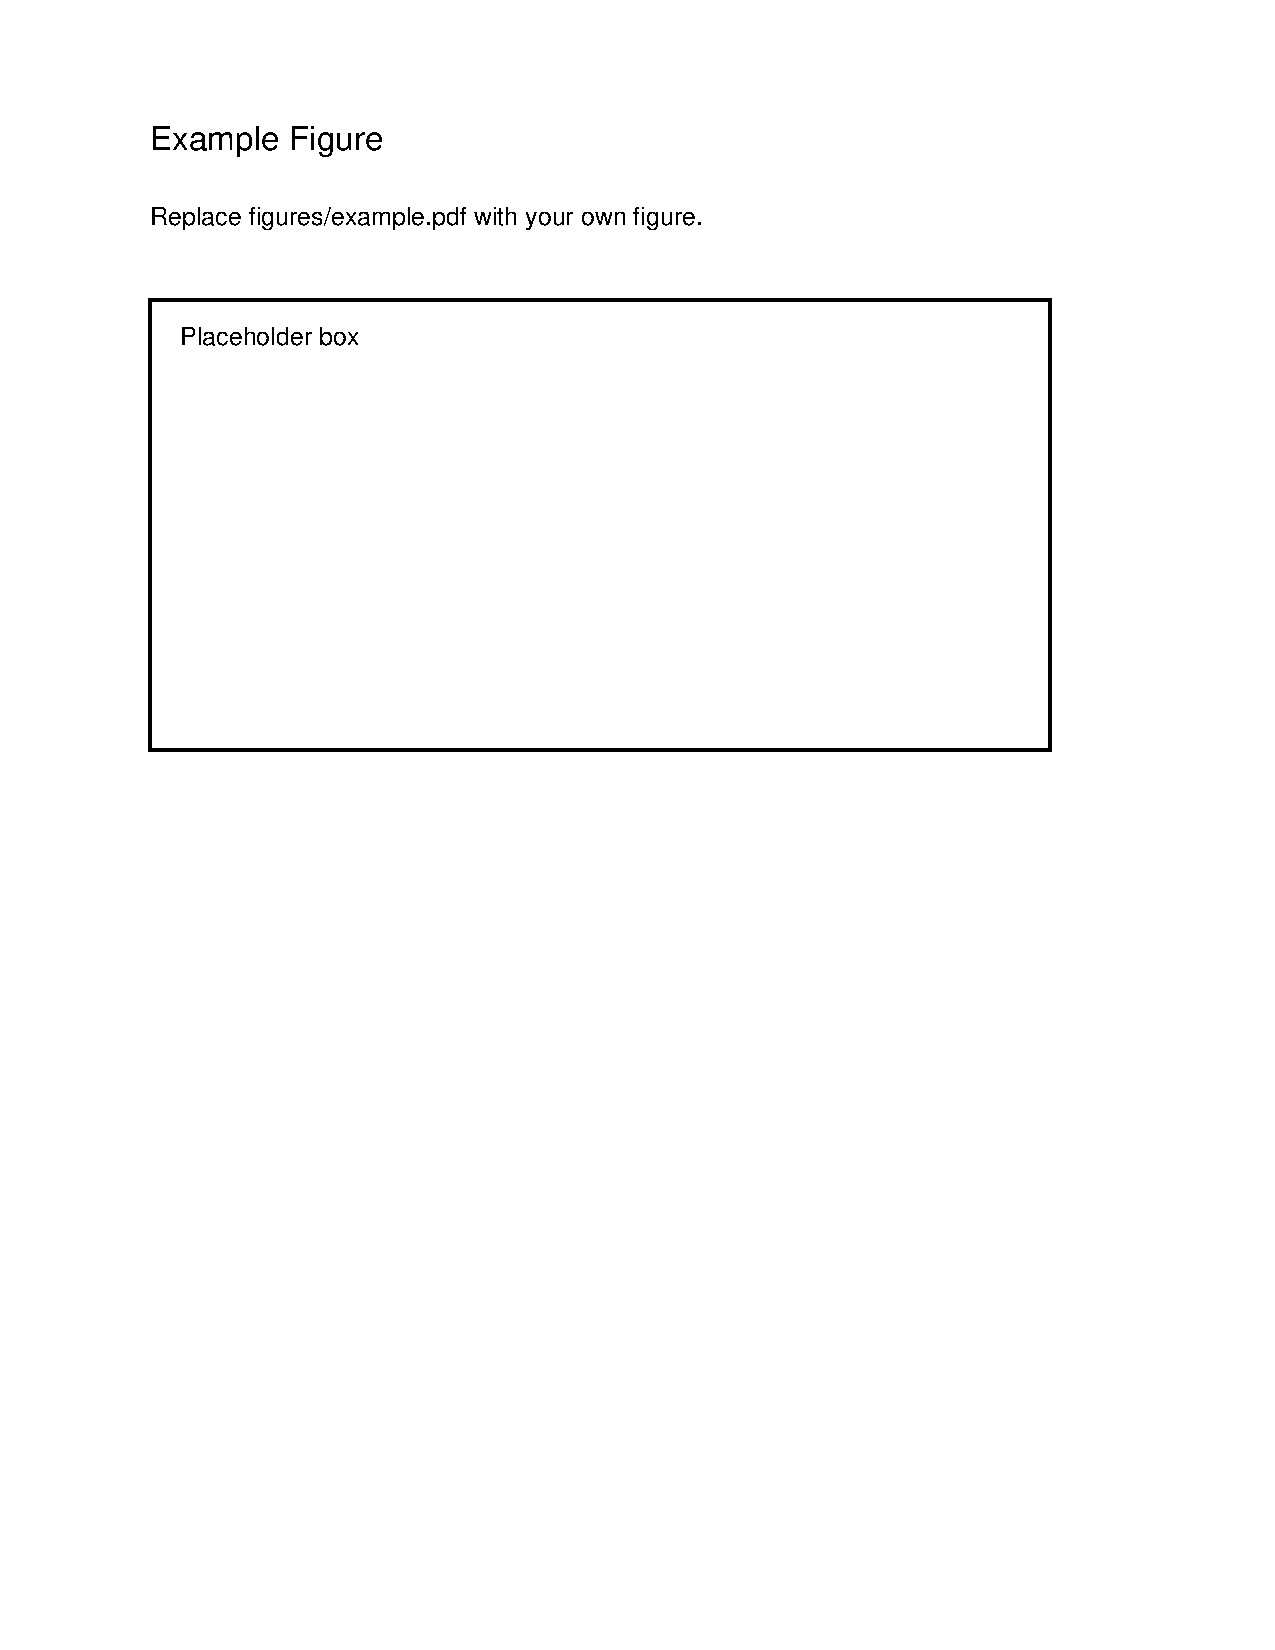
\includegraphics[width=0.65\linewidth]{figures/example.jpg}
  \caption{示例图}
  \label{fig:example}
\end{figure}

当需要展示多幅相关图像时,可采用并排或矩阵式排布方式,通过多次 \texttt{\textbackslash includegraphics} 命令实现。例如:

\begin{figure}[htbp]
  \begin{center}
    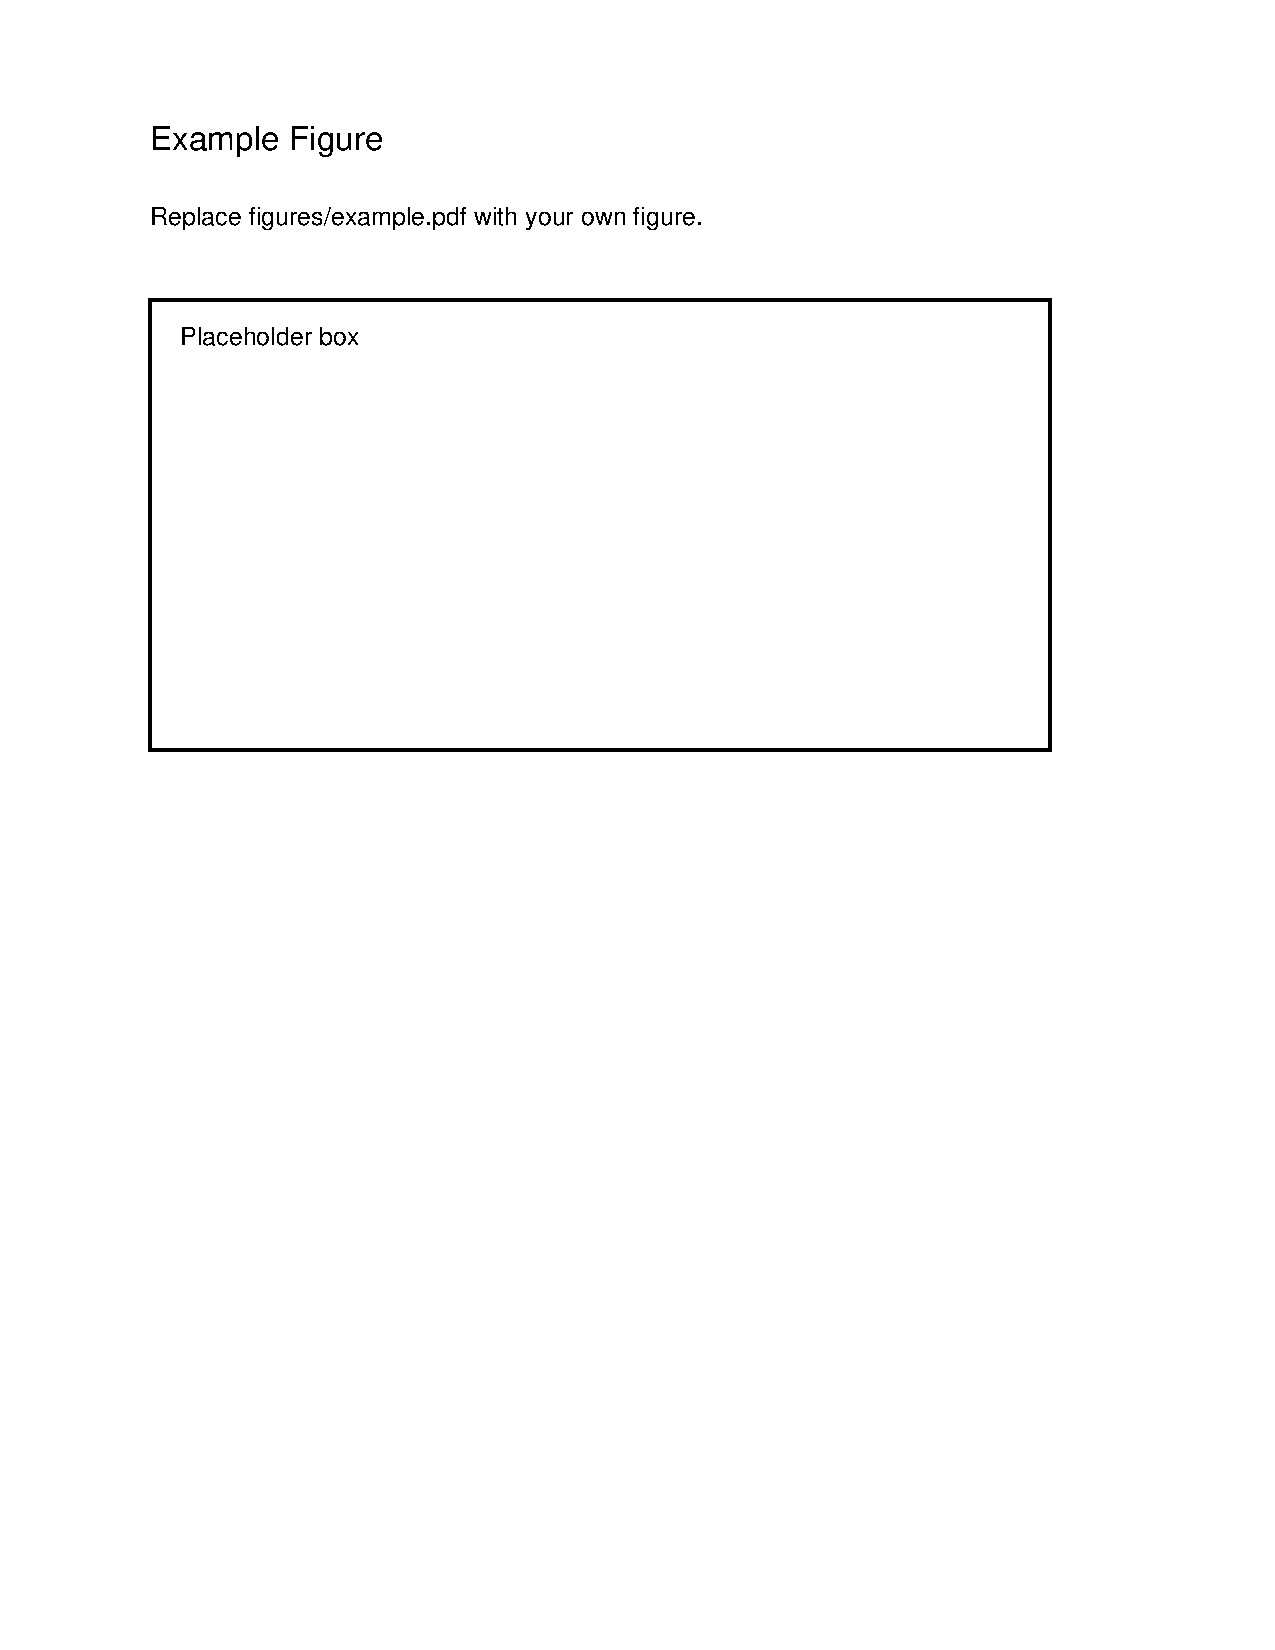
\includegraphics[width=0.45\linewidth]{figures/example.jpg}
    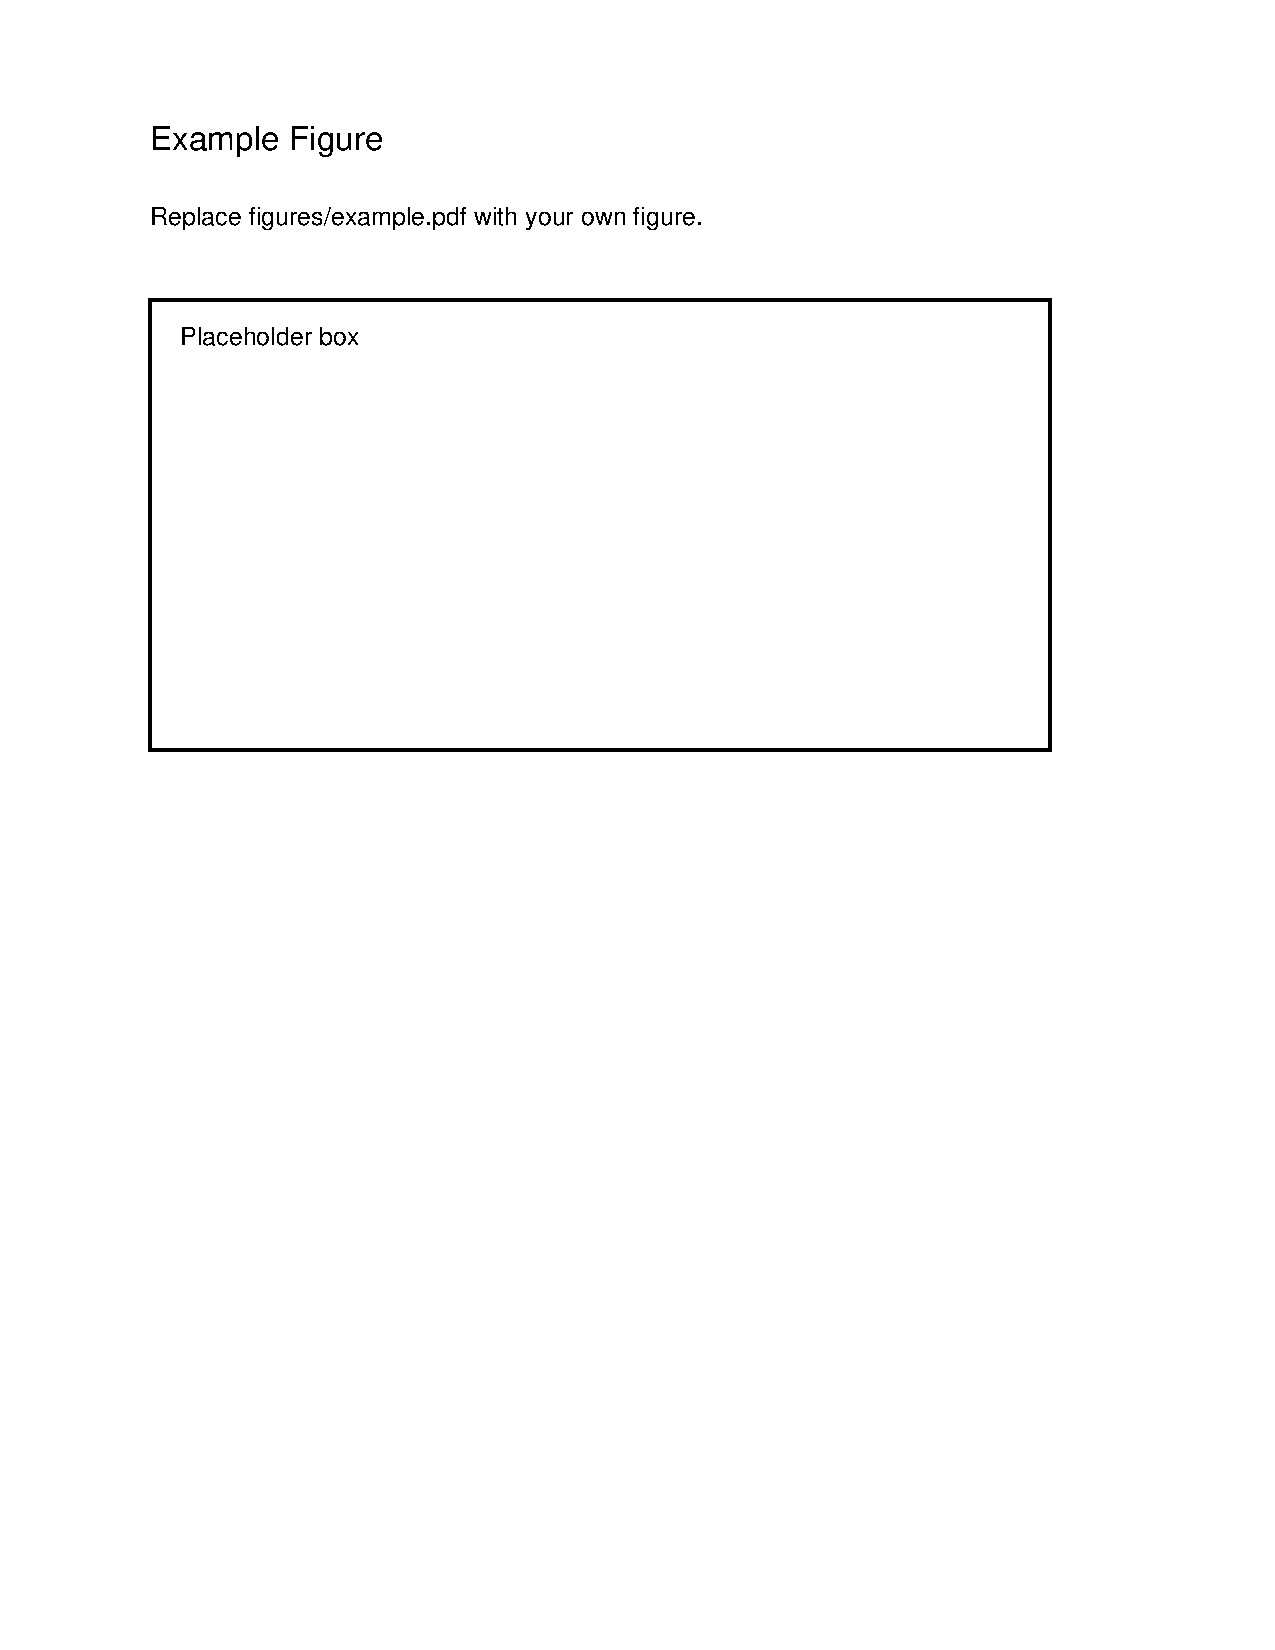
\includegraphics[width=0.45\linewidth]{figures/example.jpg}
  \end{center}
  \begin{center}
    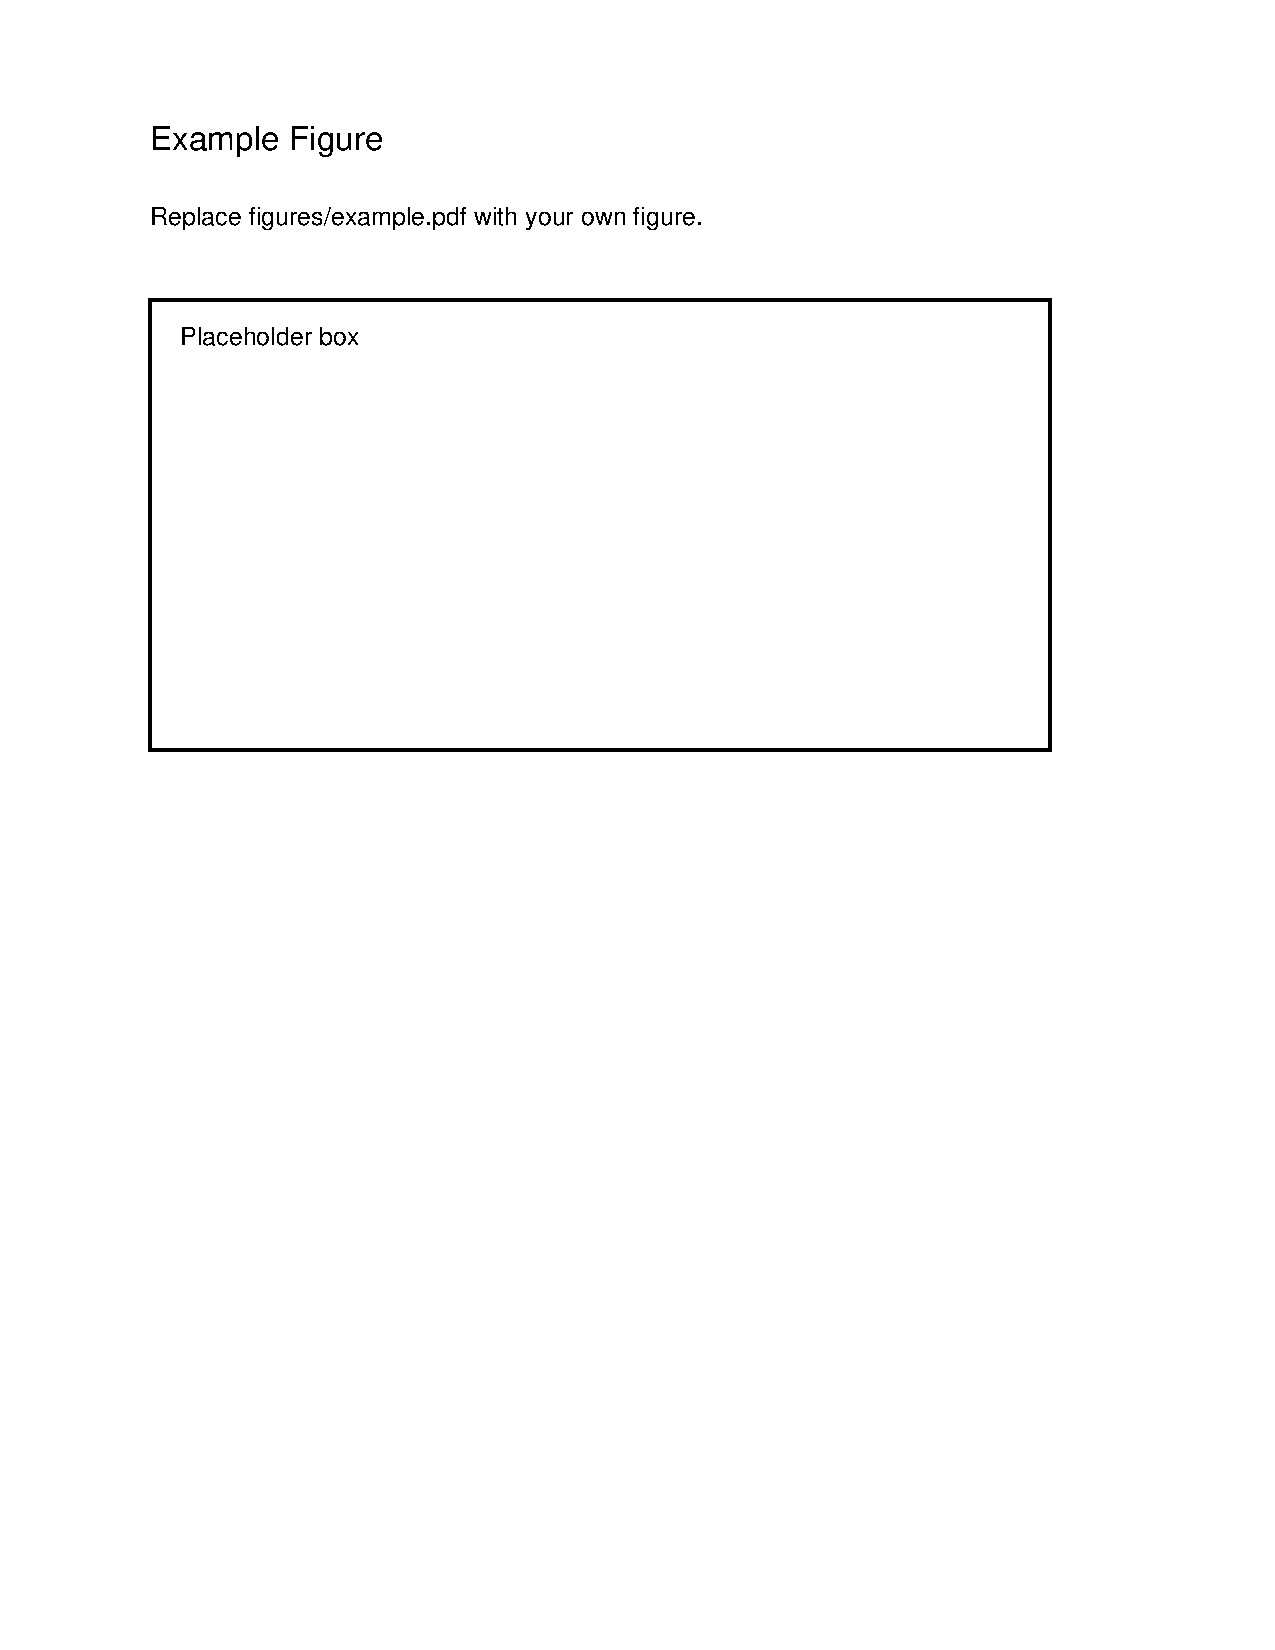
\includegraphics[width=0.45\linewidth]{figures/example.jpg}
    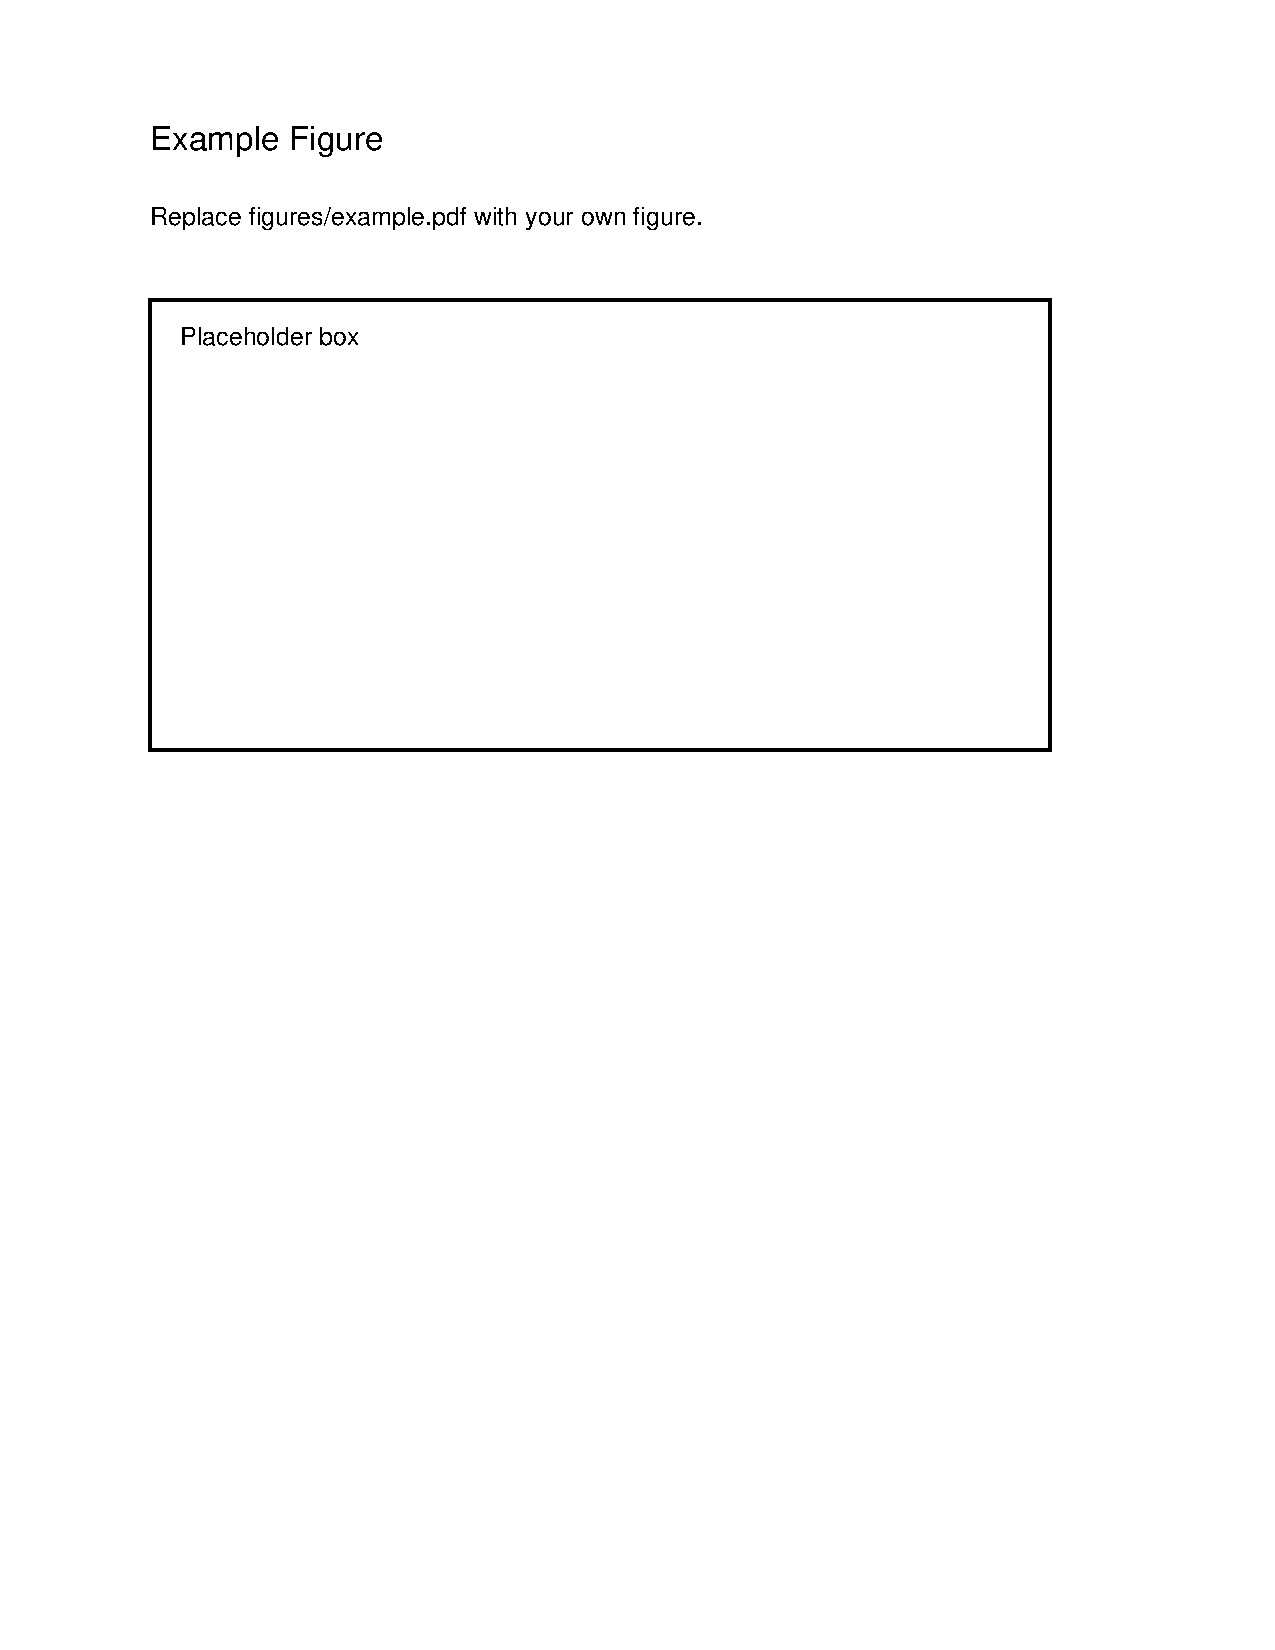
\includegraphics[width=0.45\linewidth]{figures/example.jpg}
  \end{center}
  \caption{多组图示例}
  \label{fig:aa}
\end{figure}

\begin{figure}[htbp]
  \centering
  \begin{subfigure}{\linewidth}
    \centering
    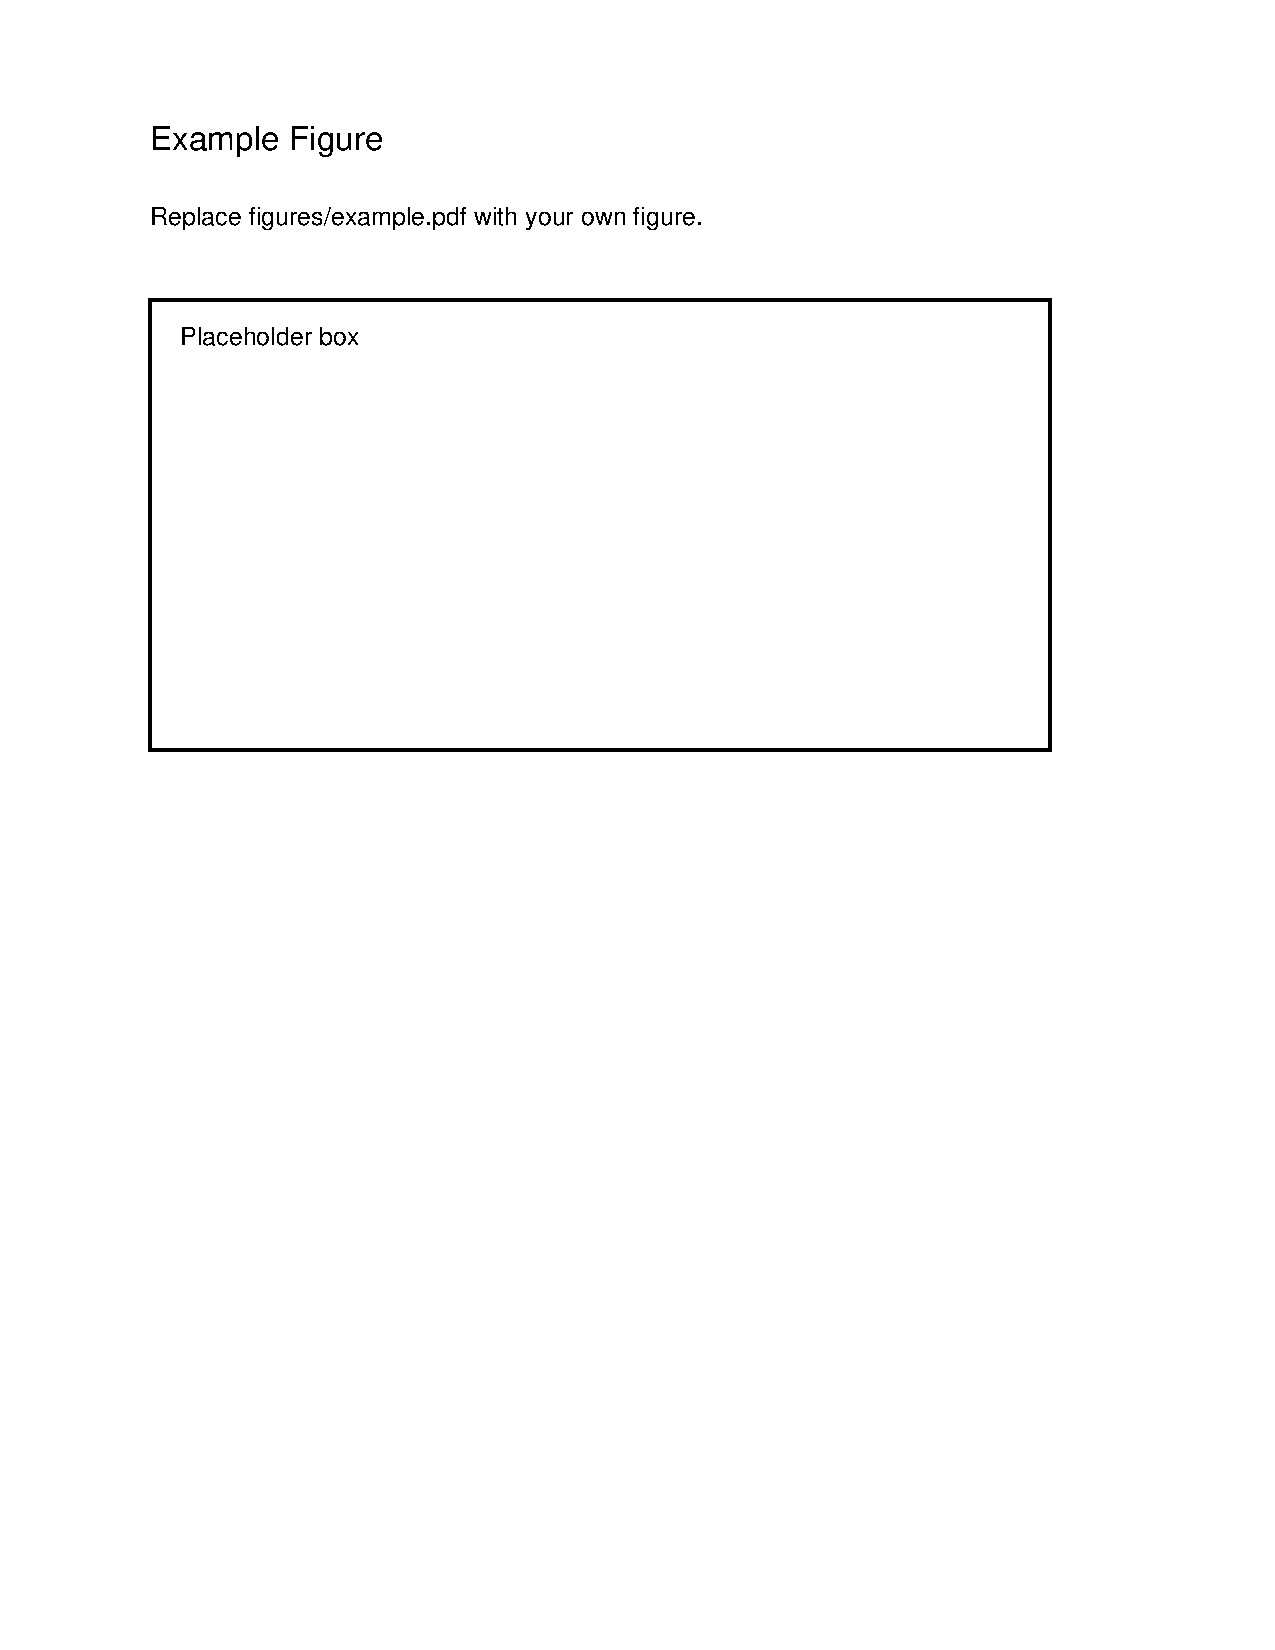
\includegraphics[width=0.45\linewidth]{figures/example.jpg}
    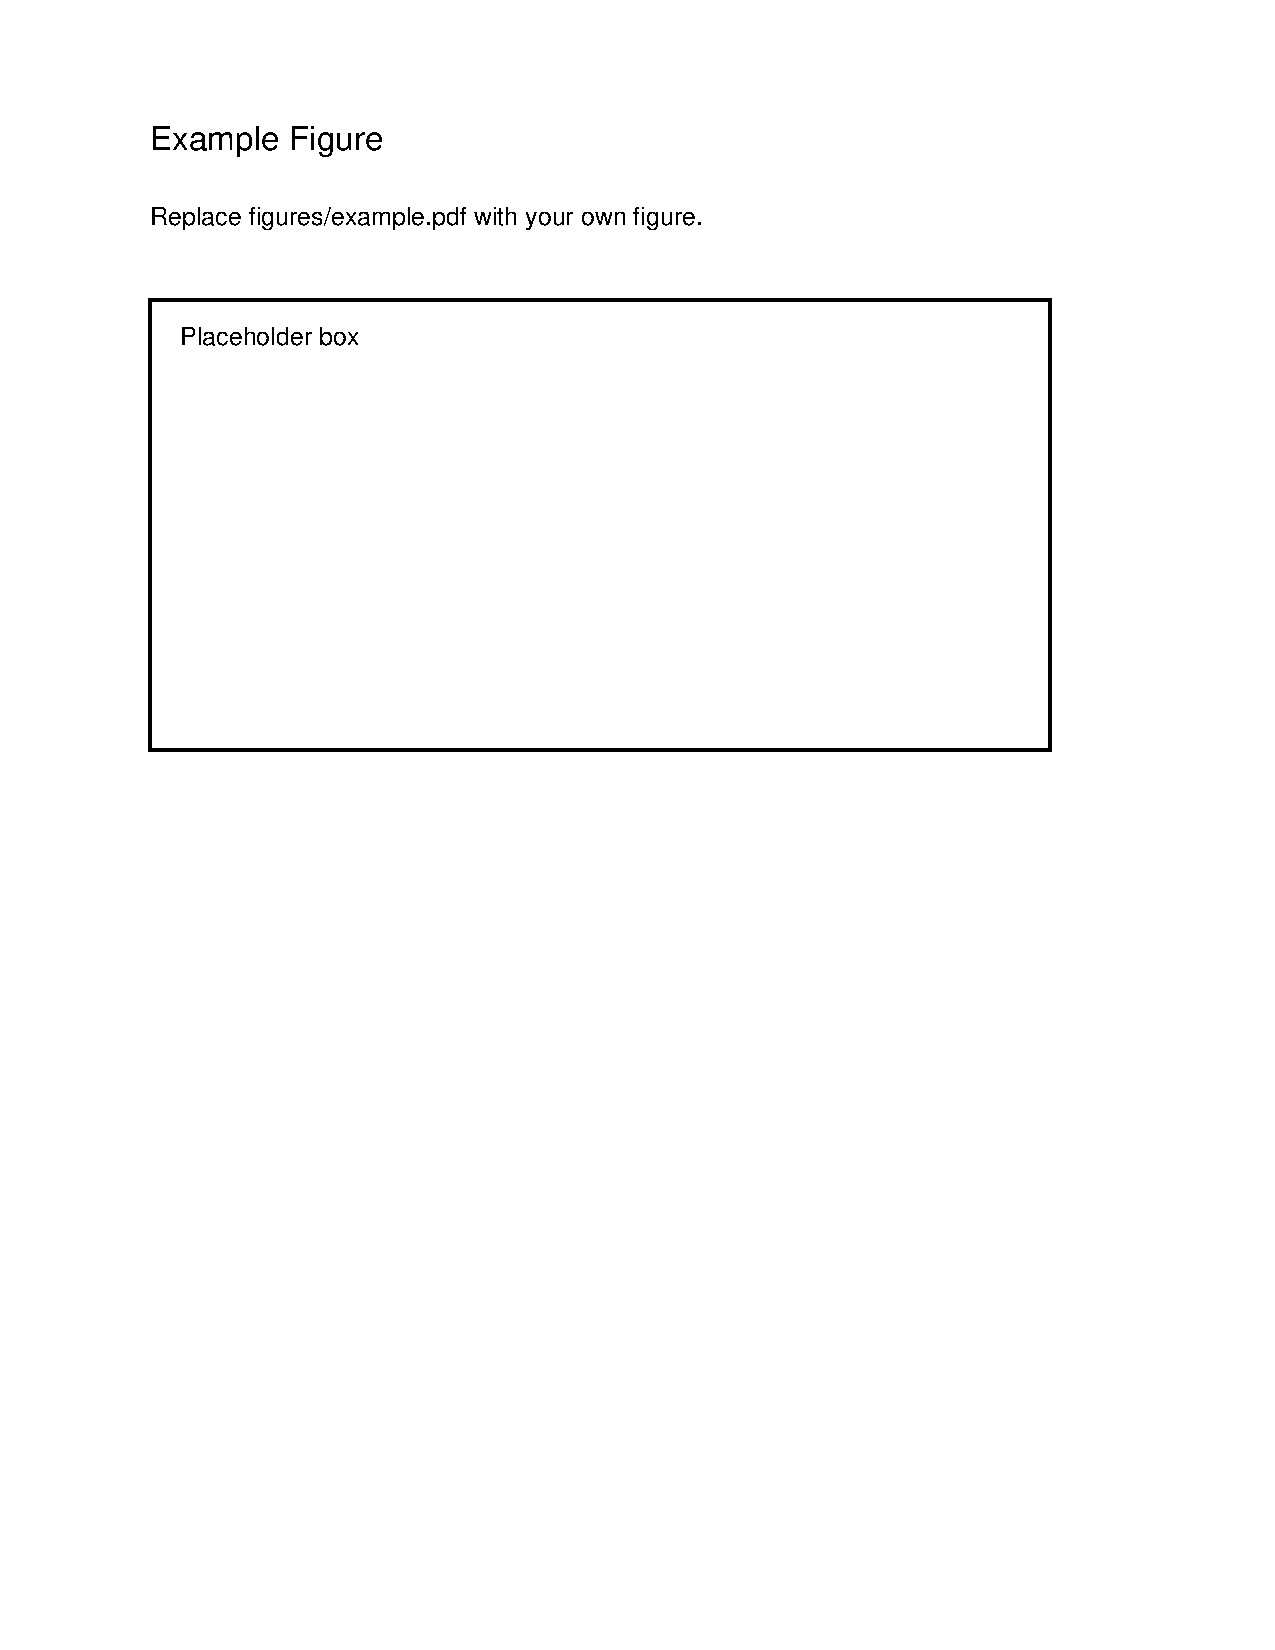
\includegraphics[width=0.45\linewidth]{figures/example.jpg}
    \caption{结果 A}
    \label{fig:a}
  \end{subfigure}
  \hfill
  \begin{subfigure}{0.45\linewidth}
    \centering
    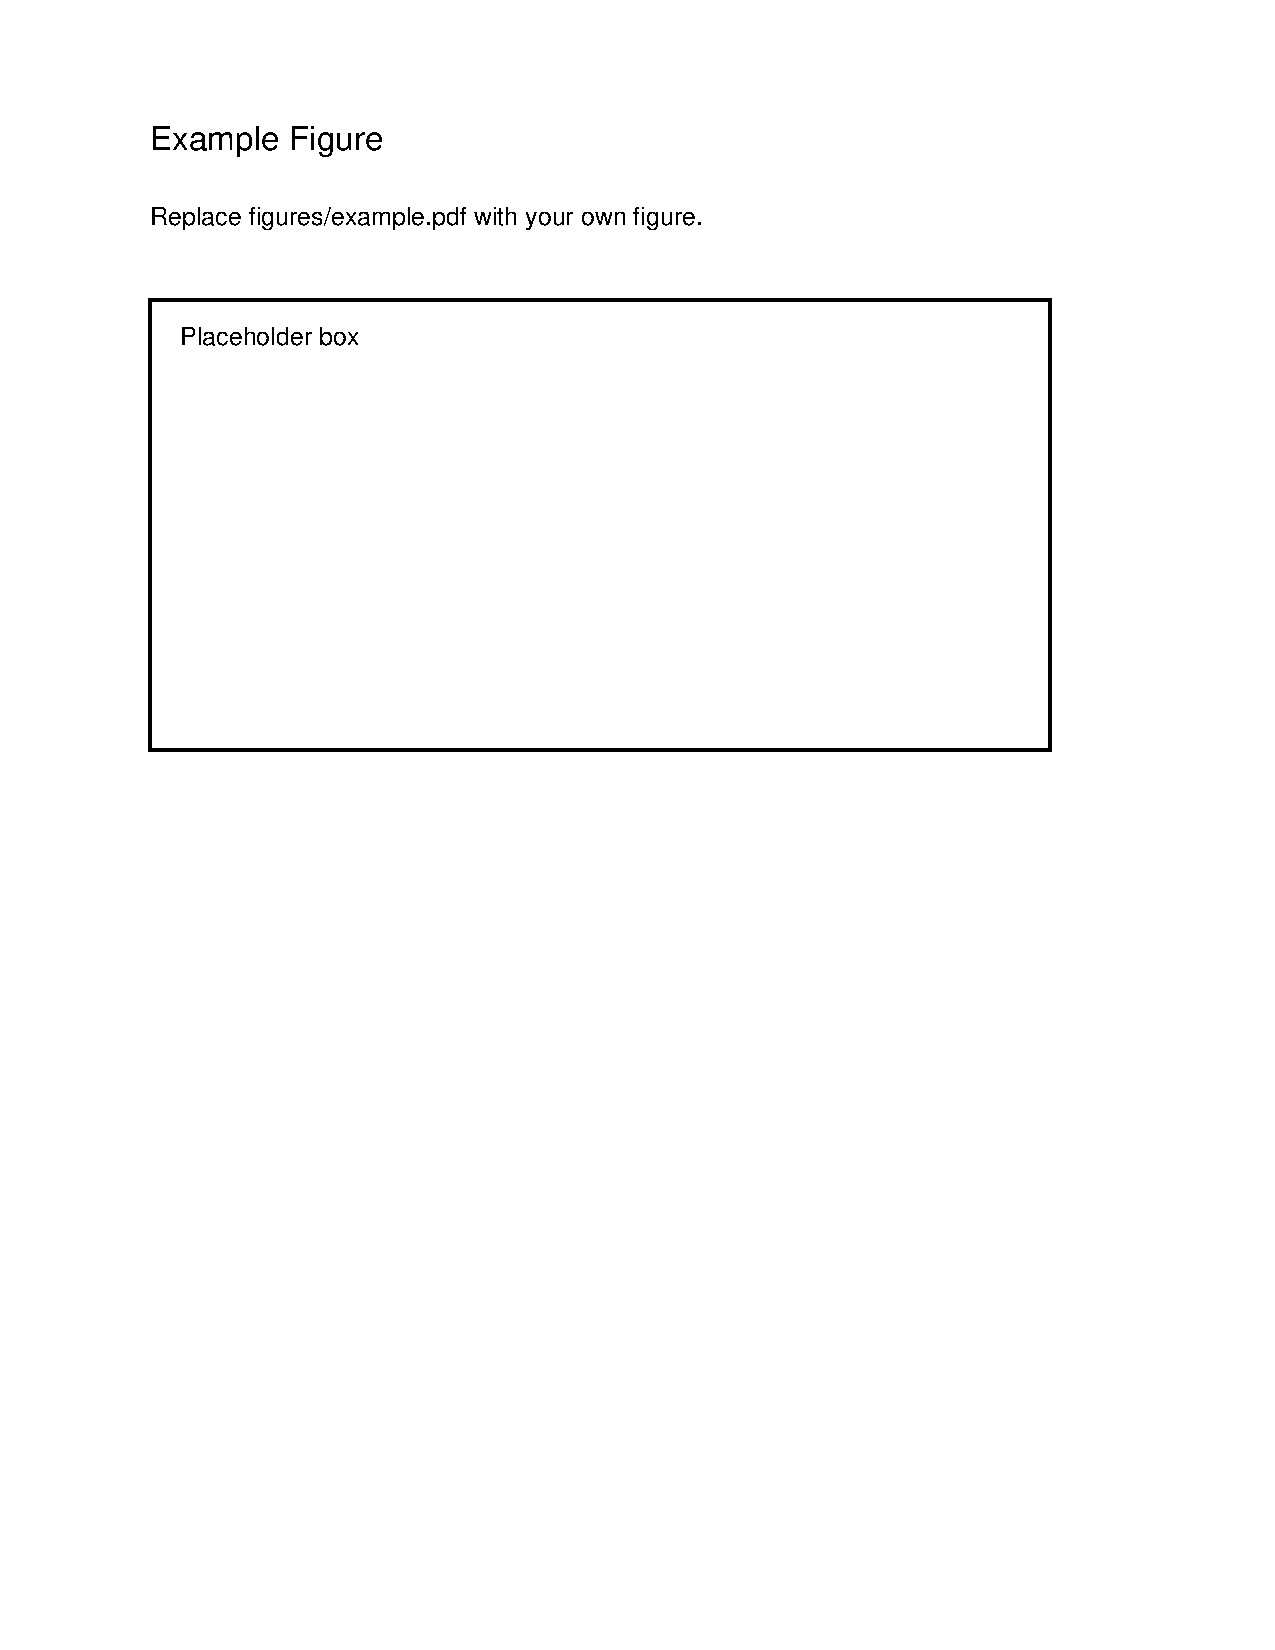
\includegraphics[width=\linewidth]{figures/example.jpg}
    \caption{结果 B}
    \label{fig:b}
  \end{subfigure}
  \caption{不同方法结果对比}
  \label{fig:ab}
\end{figure}



图题应简洁准确,能够独立说明图像内容;所有图形均应在正文中被引用后再出现。

\subsection{一般表格}

表格常用于展示实验数据、参数设置或结果对比。本模板推荐使用三线表格式排版,以增强表格的可读性和规范性。表题位于表格上方,内容示例如下:

\setlength{\tabcolsep}{20pt}
\begin{table}[htbp]
\centering
\caption{不同算法性能比较}
\label{tab:performance}
    \begin{tabular}{lccc}
    \toprule
        算法 & 准确率(\%) & 召回率(\%) & F1 值 \\ 
        \midrule
        算法 A & 92.3 & 90.1 & 91.2 \\
        算法 B & 89.7 & 88.4 & 89.0 \\
        算法 C & 94.5 & 93.2 & 93.8 \\
    \bottomrule
    \end{tabular}
\end{table}

表格中的数据应与正文分析相对应,避免仅罗列数据而缺乏说明。
\subsection{纵向表格}
纵向表格如\cref{tab:wide}所示
\begin{sidewaystable}[p]
\centering
\caption{各算法在不同数据集上的性能对比}
\label{tab:wide}
\begin{tabular}{lcccccccc}
\toprule
方法 & 指标1 & 指标2 & 指标3 & 指标4 & 指标5 & 指标6 & 指标7 & 指标8 \\
\midrule
算法A &  &  &  &  &  &  &  &  \\
算法B &  &  &  &  &  &  &  &  \\
\bottomrule
\end{tabular}
\end{sidewaystable}

\subsubsection{表格合并单元格}
表格合并单元格如\cref{tab:2-3}所示
\begin{table}[ht]
    \centering
    \caption{table:2-3}
    \label{tab:2-3}
    \begin{tabular}{llccc}
    \toprule
    \multirow{2}{*}{数据集}
    & \multirow{2}{*}{方法}
    & \multicolumn{3}{c}{指标} \\
    \cmidrule(lr){3-5}
    & & Acc & Recall & F1 \\
    \midrule
    a & a & a & a & a\\  % 每行后面都要加换行符号
    \bottomrule
    \end{tabular}

\end{table}


\section{算法}

当论文中涉及计算流程或方法步骤时,可使用算法环境进行描述。本模板支持算法自动编号与行号显示,便于表述复杂流程。

算法示例如下:

\begin{algorithm}[H]
    \caption{示例算法}
    \begin{algorithmic}[1]
        \Require 数据集 $D$
        \Ensure 模型参数 $\theta$
        \State 初始化 $\theta$
        \For{$i=1$ to $T$}
            \State 更新 $\theta$
        \EndFor
        \While{$i \le T$}
            \State While 循环
        \EndWhile
    \end{algorithmic}
\end{algorithm}

其中,\texttt{\textbackslash Require} 与 \texttt{\textbackslash Ensure} 分别用于说明算法的输入条件与输出结果。

\section{定理与证明}

对于重要的理论结论、性质或推导结果,可使用定理(Theorem)环境进行表述。模板中定理内容采用斜体排版,以突出其理论性质。

\begin{theorem}[示例定理]
若……则……
\end{theorem}

定理环境同样支持可选标题,用于对定理内容进行简要概括。

定理与证明是理论分析的重要组成部分。定理环境用于陈述结论,证明环境用于给出推导过程。模板中证明环境的“证明.”二字自动加粗,证明内容采用正体排版,格式统一。

\begin{theorem}
    \label{th:1}
    asdasd
\end{theorem}

\begin{proof}
    dsas
\end{proof}

作者在书写证明时,无需额外添加格式命令,仅需关注逻辑推导过程。

\section{引用}

论文中涉及的文献应统一通过 Bib\TeX{} 管理,并在正文中使用引用命令进行标注。例如:

文献引用示例:\cite{example2024paper}

对于定理、公式等对象,建议使用交叉引用方式进行说明:

定理引用方式一:\cref{th:1},方式二:\ref{th:1}。

对于不需要编号的公式,可使用无编号公式环境:

\begin{equation*}
    a = b
\end{equation*}

需要编号的公式使用如下形式:

\begin{equation}
    \label{eq:2}
    a = b
\end{equation}

公式引用方式一:\ref{eq:2},方式二:\cref{eq:2}。

\section{插入代码}

\begin{lstlisting}[language=Java, caption={MapReduce 主流程}, label={lst:mr}]
public static void main(String[] args) {
    System.out.println("Hello, Hist!");
}
\end{lstlisting}




\chapter{结论与展望}

\section{研究结论}
总结主要贡献(建议条理化)。
本文采用 \kw{Branch-and-Bound} 算法进行求解。
\section{不足与未来工作}
给出局限与展望。


%====================== 参考文献 ======================%
% \printbibliography[heading=bibliography,title={参考文献}]
% \addcontentsline{toc}{chapter}{参考文献}

%====================== 参考文献(BibTeX) ======================%
\cleardoublepage
\phantomsection
\addcontentsline{toc}{chapter}{参考文献}

\begingroup
% \setlength{\baselineskip}{0pt}   % ← 关键:压缩文献内部行距
% \setlength{\bibsep}{6pt}          % 条目之间不额外加空
% \setlength{\parskip}{0pt}
\renewcommand{\baselinestretch}{1}\selectfont % 可选:让参考文献行距别跟正文固定行距走
\bibliography{\HISTbibname}
\endgroup
% \bibliography{references}

%====================== 附录、致谢、成果 ======================%
\ifShowAppendix
  \appendix
  % 附录在这里引入
  \chapter{补充推导与实验细节}

这里放证明、额外实验、代码片段说明等。

  
\fi

\chapter*{致谢}\markboth{致谢}{}
% \addcontentsline{toc}{chapter}{致谢}
祝大家以梦为马,不负韶华!

愿大家出走半生,归来仍是少年!
\chapter*{攻读学位期间取得的成果}\markboth{攻读学位期间取得的成果}{}
% \addcontentsline{toc}{chapter}{攻读学位期间取得的成果}
\begin{enumerate}
  \item 论文:作者. 题目[J]. 期刊, 年, 卷(期): 页码.
  \item 专利:发明人. 专利名称: 专利号[P]. 年-月-日.
\end{enumerate}

\end{document}
